\subsection{Field}
"Field" klassen er en abstrakt klasse, dvs. at den ikke er implementeret. Klassen er abstrakt da der i spillet bliver anvendt mange forskellige slags felter, der mere eller mindre har de samme egenskaber, dog med enkelte variationer. Der er derfor mulighed for at oprette felt klasser der passer speficikt til den type der skal laves. "Field" klassen indeholder en række "standard" metoder som f.eks. en konstruktør (figur \ref{fig:fieldKons}) og en toString() metode (figur \ref{fig:fieldString}).

\begin{figure}[H]
    \centering
    \includegraphics[width=17cm]{sources/7_implementering/fieldkonstruktør.PNG}
    \caption{Field klassens konstruktør}
    \label{fig:fieldKons}
\end{figure}
\begin{figure}[H]
    \centering
    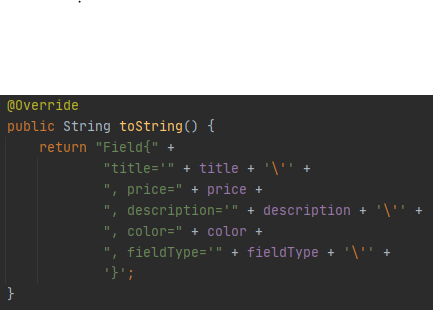
\includegraphics{sources/7_implementering/fieldTostring.PNG}
    \caption{Field klassens toString metode}
    \label{fig:fieldString}
\end{figure}

